% ^
\documentclass[addpoints,spanish, 12pt,a4paper]{exam}
%\documentclass[answers, spanish, 12pt,a4paper]{exam}
\printanswers
\pointpoints{punto}{puntos}
\hpword{Puntos:}
\vpword{Puntos:}
\htword{Total}
\vtword{Total}
\hsword{Resultado:}
\hqword{Ejercicio:}
\vqword{Ejercicio:}

\usepackage[utf8]{inputenc}
\usepackage[spanish]{babel}
\usepackage{eurosym}
%\usepackage[spanish,es-lcroman, es-tabla, es-noshorthands]{babel}


\usepackage[margin=1in]{geometry}
\usepackage{amsmath,amssymb, cancel}
\usepackage{multicol}
\usepackage{yhmath}

\pointsinrightmargin % Para poner las puntuaciones a la derecha. Se puede cambiar. Si se comenta, sale a la izquierda.
\extrawidth{-2.4cm} %Un poquito más de margen por si ponemos textos largos.
\marginpointname{ \emph{\points}}

\usepackage{graphicx}

\graphicspath{{../img/}} 

\newcommand{\class}{2º Bachillerato CCSS}
\newcommand{\examdate}{\today}
\newcommand{\examnum}{Final 2ªEv.}
\newcommand{\tipo}{A}


\newcommand{\timelimit}{105 minutos}

\renewcommand{\solutiontitle}{\noindent\textbf{Solución:}\enspace}


\pagestyle{head}
\firstpageheader{
\includegraphics[width=0.2\columnwidth]{header_left}}{\textbf{Departamento de Matemáticas\linebreak \class}\linebreak \examnum}{
\includegraphics[width=0.1\columnwidth]{header_right}}
\runningheader{\class}{\examnum}{Página \thepage\ of \numpages}
\runningheadrule


\usepackage{pgf,tikz,pgfplots}
\pgfplotsset{compat=1.15}
\usepackage{mathrsfs}
\usetikzlibrary{arrows}


\begin{document}

\noindent
\begin{tabular*}{\textwidth}{l @{\extracolsep{\fill}} r @{\extracolsep{6pt}} }
\textbf{Nombre:} \makebox[3.5in]{\hrulefill} & \textbf{Fecha:}\makebox[1in]{\hrulefill} \\
 & \\
\textbf{Tiempo: \timelimit} & Tipo: \tipo 
\end{tabular*}
\rule[2ex]{\textwidth}{2pt}
Esta prueba tiene \numquestions\ ejercicios. La puntuación máxima es de \numpoints. 
La nota final de la prueba será la parte proporcional de la puntuación obtenida sobre la puntuación máxima. 

\begin{center}


\addpoints
 %\gradetable[h][questions]
	\pointtable[h][questions]
\end{center}

\noindent
\rule[2ex]{\textwidth}{2pt}

\begin{questions}

\question[4] Calcula los siguientes límites:
\begin{parts}

%https://academico.unizar.es/sites/academico.unizar.es/files/enviodocumento/acceso/armon/matemaplic/acta20191021.pdf

\part $\lim_{x \to 0}\frac{x+1}{x-1}$
\begin{solution}$-1$\end{solution}
\part $\lim_{x \to +\infty}(\sqrt{x}-\sqrt{x-1})$
\begin{solution}$-1$\end{solution}
\part $\lim_{x \to 1}\frac{1}{\ln x}$
\begin{solution}$ \nexists$\end{solution}
\part $\lim_{x \to 0^+}\ln x$
\begin{solution}$-\infty$\end{solution}
% \part $\lim_{x \to +\infty}e^{x+1}$
% \begin{solution}$\infty$\end{solution}
% \part $\lim_{x \to +\infty}\frac{x^2+\sqrt{x+1}}{7x^2-x+4}$
% \begin{solution}$\frac{1}{7}$\end{solution}

\end{parts}

% para comentar ctrl+/ o ctrl+shift+7

\question \textbf{Sept. 12} Calcular las derivadas de las siguientes funciones: 
\begin{parts}
\part[1] $f(x)=\frac{1}{x}+2\ln x - \frac{\ln x}{x}$
\begin{solution}
$\frac{2}{x} + \frac{1}{x^{2}} \ln{\left (x \right )} - \frac{2}{x^{2}}=\frac{1}{x^{2}} \left(2 x + \ln{\left (x \right )} - 2\right)$
\end{solution}
\part[1] $g(x)=\dfrac{e^x}{(x-1)^2}$
\begin{solution}
$\frac{\left(- 2 x + 2\right) e^{x}}{\left(x - 1\right)^{4}} + \frac{e^{x}}{\left(x - 1\right)^{2}}=\frac{e^{x}}{\left(x - 1\right)^{4}} \left(- 2 x + \left(x - 1\right)^{2} + 2\right)$

\end{solution}
\end{parts}

\question[4] Calcula las siguientes integrales:
\begin{parts}
\part $\int \left(x^2+5x+\frac{1}{x} \right) dx$
\begin{solution}
 $\int \left(x^{2} + 5 x + \frac{1}{x}\right)\, dx=\frac{x^{3}}{3} + \frac{5 x^{2}}{2} + \ln{\left (x \right )}+ C $   
\end{solution}
\part $\int \dfrac{1}{(x+2)^3} dx$
\begin{solution}
   $\int \frac{1}{\left(x + 2\right)^{3}}\, dx=- \frac{1}{2 x^{2} + 8 x + 8}+ C $  
\end{solution}
\part $\int \dfrac{x+7}{x^2} dx$
\begin{solution}
 $\int \frac{1}{x^{2}} \left(x + 7\right)\, dx=\ln{\left (x \right )} - \frac{7}{x}+ C $
\end{solution}
\part $\int \dfrac{7x}{\sqrt{x^2+1}} dx$
\begin{solution}
  $\int \frac{7 x}{\sqrt{x^{2} + 1}}\, dx=7 \sqrt{x^{2} + 1}+ C $ 
\end{solution}

\end{parts}

\question[2] \textbf{Sept. 12} Calcular $$\int_0^2 (4x^3+e^{3x}) dx$$
\begin{solution}
$\int_{0}^{2} \left(4 x^{3} + e^{3 x}\right)\, dx=\left[x^{4} + \frac{e^{3 x}}{3}\right]_{0}^2=\frac{47}{3} + \frac{e^{6}}{3}$
\end{solution}

\question    \textbf{Sept. 12} Se ha realizado una encuesta a una determinada población con el fin de determinar el número de personas que utilizarían el sistema de autobuses si la tarifa admitiera distintos importes. Basándose en los resultados de las encuestas, los analistas de sistemas han determinado una función aproximada que expresa el número diario de pasajeros en función de la tarifa. La función demanda viene dada por $D(x)=\sqrt{10+3x-\frac{5}{4}x^2} $, donde $x$ representa la tarifa en euros.


\begin{parts}
\part[2] ¿Qué tarifa habrá que aplicar para obtener el mayor número de pasajeros? 
\begin{solution}
$f'(x)=\frac{- \frac{5 x}{4} + \frac{3}{2}}{\sqrt{- \frac{5 x^{2}}{4} + 3 x + 10}}=\frac{- 5 x + 6}{2 \sqrt{- 5 x^{2} + 12 x + 40}}$ \\
$f''(x)=\frac{\left(- \frac{5 x}{4} + \frac{3}{2}\right) \left(\frac{5 x}{4} - \frac{3}{2}\right)}{\left(- \frac{5 x^{2}}{4} + 3 x + 10\right)^{\frac{3}{2}}} - \frac{5}{4 \sqrt{- \frac{5 x^{2}}{4} + 3 x + 10}}=- \frac{118}{\left(- 5 x^{2} + 12 x + 40\right)^{\frac{3}{2}}}$\\
$f'(x)=0 \to x=\frac{6}{5}$ \\
$f''(\frac{6}{5})= - \frac{5 \sqrt{295}}{236} < 0 \to max$ \\
La tarifa debe ser de 1,20\euro  para obtener el mayor número de pasajeros.
\end{solution}
\part[1] Si la tarifa aplicada está entre 1 y 2 euros, ¿cómo es la variación en la afluencia de pasajeros? ¿Creciente, decreciente? 
\begin{solution}
Entre 1 y 1,20 euros, la afluencia de pasajeros será creciente. Entre 1,20 y 2 euros, la afluencia será 
decreciente.

\end{solution}
\end{parts}

\question \textbf{Jun. 12} Considerar la función $f(x)= \begin{cases} \dfrac{x-3}{(x-4)(x-5)} &  x \leq 3 \\ \dfrac{x^2-2}{(x+1)(x+3)} & x>3 \end{cases}$

\begin{parts}
\part[1] Estudiar la continuidad de $f(x)$ en $x=3$
\begin{solution}
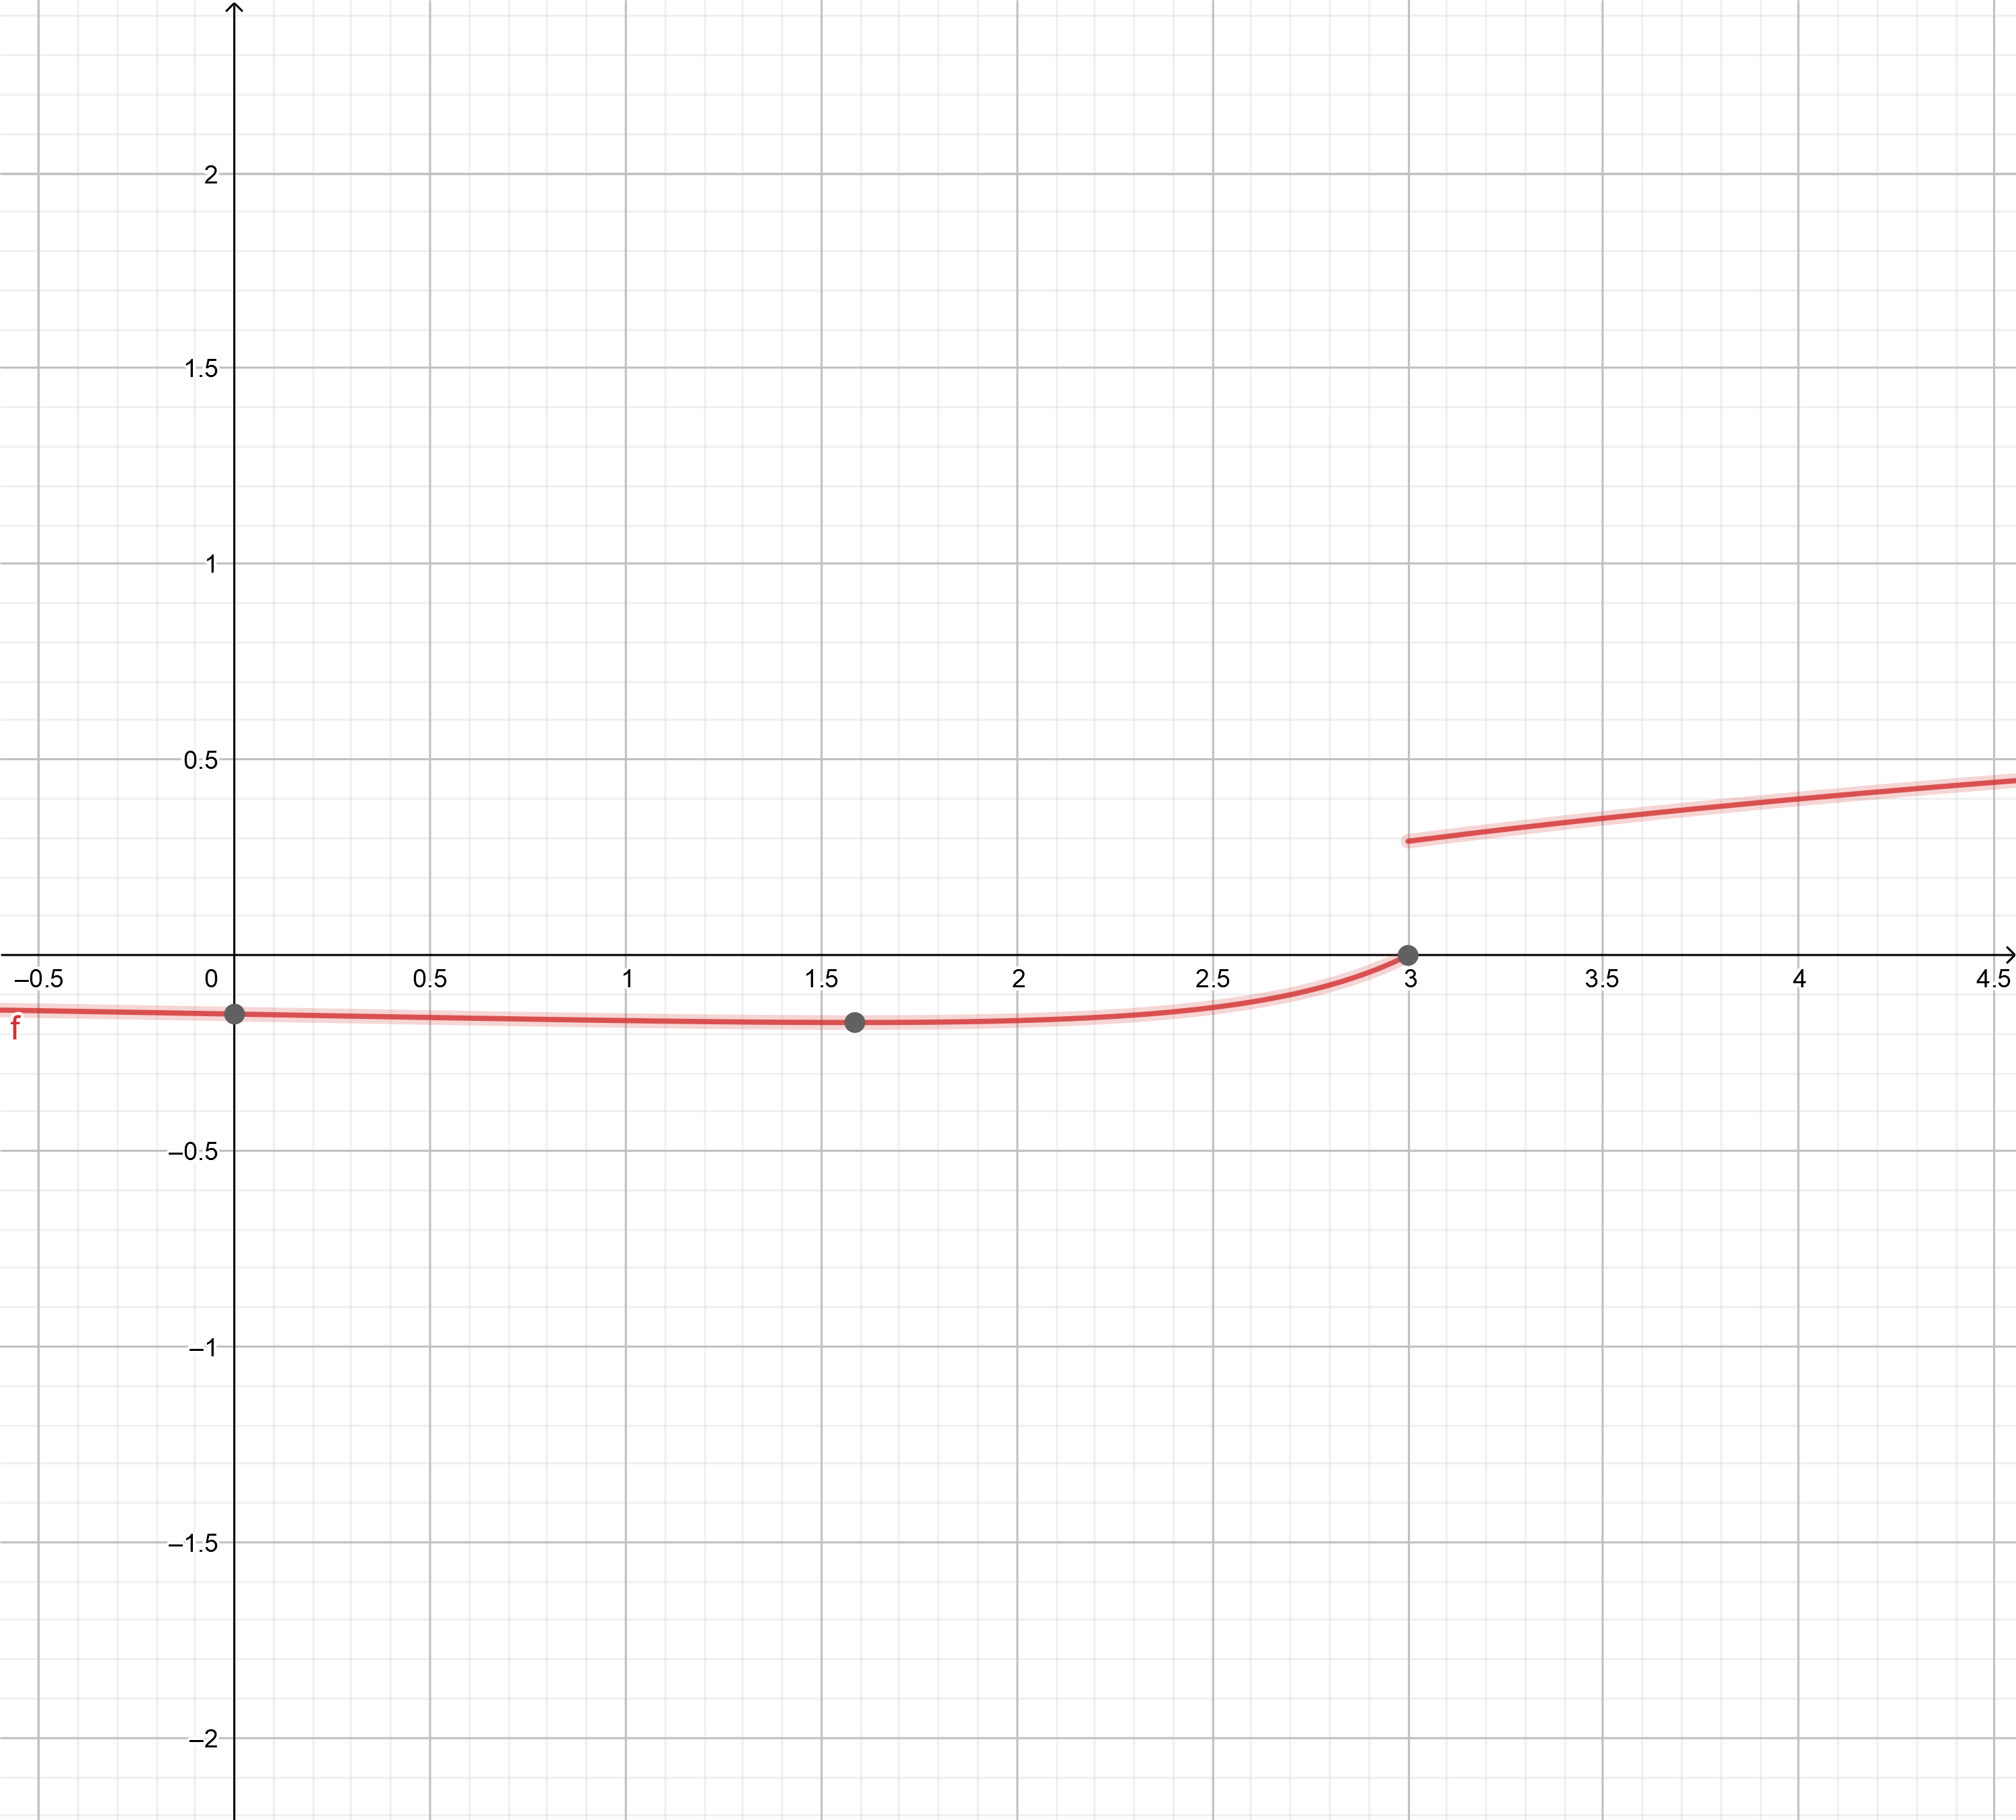
\includegraphics[scale=1]{tex/fi2_1.png} \\
Singularidades de las expresiones analíticas: $\emptyset$.\\ Posibles discontinuidades en los extremos de los trozos:3.\\En 3 no es continua porque no existe límite. Límites laterales: $0$ y $\frac{7}{24}$
\end{solution}
\part[2] Hallar los intervalos de crecimiento y decrecimiento de $f(x)$ así como los máximos y mínimos si $x\leq3$
\begin{solution} 
$f(x)= \frac{x - 3}{\left(x - 5\right) \left(x - 4\right)}$\\
$f'(x)=\frac{1}{\left(x - 5\right) \left(x - 4\right)} - \frac{x - 3}{\left(x - 5\right) \left(x - 4\right)^{2}} - \frac{x - 3}{\left(x - 5\right)^{2} \left(x - 4\right)}=- \frac{x^{2} - 6 x + 7}{\left(x - 5\right)^{2} \left(x - 4\right)^{2}} \to f'(x)= 0 \Longleftrightarrow x \in \left [ - \sqrt{2} + 3, \quad \bcancel{\sqrt{2} + 3}\right]$\\
Crecimiento: $ \left(- \sqrt{2} + 3, 3\right] $ \\ 
Decrecimiento: $ \left(-\infty, - \sqrt{2} + 3\right) $ \\  
Extremos absolutos en $\left( -\infty, 3 \right ]$: \\
$f(-\infty)=0$ \\
$f(3-\sqrt{2})=-0.17$ \\
$f(3)=0$

Por tanto: $\left [ - \sqrt{2} + 3, \quad min \ rel \ y \ abs \right ], \quad \left [ 3, \quad max \  abs\right ]$
\end{solution}
\end{parts}


\question \textbf{Sept. 11} Dada la función $f(x)=\dfrac{\ln x}{x}$:

\begin{parts}
\part[1] Determine el dominio de definición
\begin{solution}
    $Dom(f)=\left(0, \infty\right)$\\
    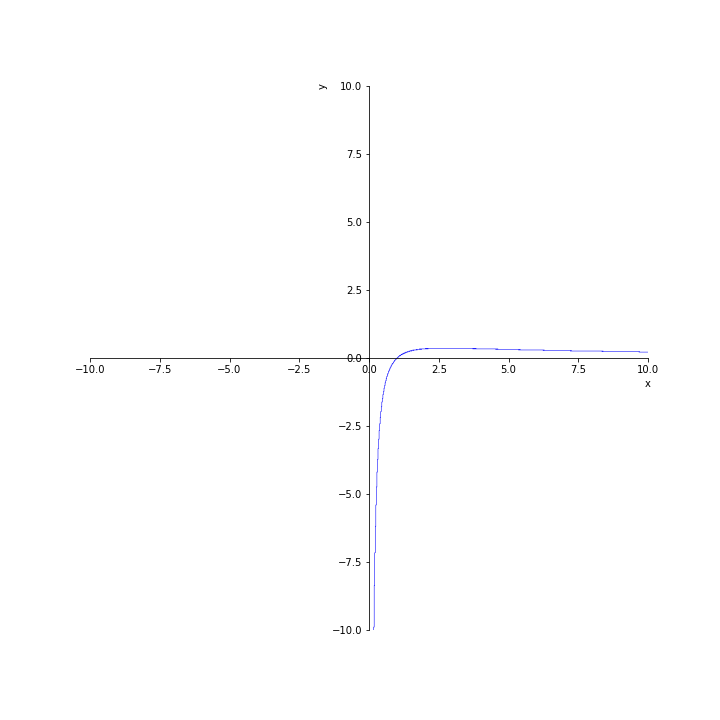
\includegraphics[scale=0.2]{fi2_2.png}
\end{solution}
\part[2] Halle sus intervalos de concavidad y convexidad así como sus puntos de inflexión.
\begin{solution}
    $f'(x)= \frac{1}{x^{2}} \left(- \ln{\left (x \right )} + 1\right)$\\
    $f''(x)=\frac{1}{x^{3}} \left(2 \ln{\left (x \right )} - 3\right)$\\
    $f''(x)=0 \Longleftrightarrow x = e^{\frac{3}{2}} \approx 4.48168907033806$\\
    $x \in (0,e^{\frac{3}{2}}) \to f''(x)<0 \to CONCAVA$\\
    $x \in (e^{\frac{3}{2}},\infty) \to f''(x)>0 \to CONVEXA$\\
    En $x=e^{\frac{3}{2}}$ hay un punto de inflexión
\end{solution}

\end{parts}

\question[1] \textbf{Sept. 01} Dada la función $$f(x)=x^3-6x^2+8x$$ 
Probar que la recta $y =-x$ es tangente a la curva $y = f(x)$  en algún punto
\begin{solution}
    $f'(x)=3 x^{2} - 12 x + 8 \land y=-x \to m=-1$\\
    $3 x^{2} - 12 x + 8=-1 \to x=1, \ x=3 \to (1,3) \land (3,-3) \to (3,-3)$

\end{solution}



\addpoints
\end{questions}

\end{document}

%\grid

